\documentclass[a4paper,12pt]{article}
\usepackage{natbib,epsfig,rotating,longtable,url,amsmath}
\usepackage{varioref}
%% font
%%\usepackage{mathptmx}
\graphicspath{{figs/}}

\begin{titlepage}
\title{Visualisation of SPH data using SUPERSPHPLOT - v\input{version}}
\author{Daniel Price}
\end{titlepage}

\begin{document}
\maketitle
\tableofcontents
\newpage

\section{Introduction}
 Whilst many wonderful commercial software packages exist for visualising scientific
data (such as the widely used Interactive Data Language), I found that such packages
could be somewhat cumbersome for the manipulation and visualisation of my SPH data. The
main problem was that much of what I wanted to do was fairly specific to SPH (such as
interpolation to an array of pixels using the kernel) and whilst generic routines exist
for such tasks, I could not explain how they worked, nor were they
particularly fast and whilst interactive gizmos are handy, it can prove more difficult to perform the
same tasks non-interactively, as required for the production of animations. 
In fact I have found that the major
work in the visualisation of SPH data is not the image production itself but the
manipulation of data prior to plotting. Much of this manipulation makes sense
within an SPH framework (for example the interpolation provided by the kernel
and rotation of the particles for perspective).

 SUPERSPHPLOT is designed for this specific task - to use SPH tools to analyse SPH data and to make this a
straightforward task such that publishable images and animations can be obtained
as efficiently as possible from the raw data with a minimum amount of effort
from the user. I have found in the process that the development of powerful
visualisation tools has enabled me to pick up on effects present in my
simulation results that I would not otherwise have noticed (in particular the
difference between a raw particle plot and a rendered image can be substantial). Part of the goal of
SUPERSPHPLOT is to eliminate the use of crap-looking particle plots as a means of representing SPH data!

\subsection{What it does}
SUPERSPHPLOT is a utility for visualisation of output from (astrophysical) simulations using the
Smoothed Particle Hydrodynamics (SPH) method in one, two and three dimensions.
It is written in Fortran 90/95 and
utilises PGPLOT subroutines to do the actual plotting. In particular the following
features are included:
\begin{itemize}
\item Rendering of particle data to an array of pixels using the SPH kernel
\item Cross-sections through 2D and 3D data (as both particle plots and rendered
images).
\item Fast projections through 3D data (ie. column density plots, or integration of
other quantities along the line of sight)
\item Vector plots of the velocity (and other vector quantities), including vector
plots in a cross section slice in 3D.
\item Rotation and fly-throughs (multiple cross-section slices) of 3D data.
\item Automatic stepping through timesteps, making animations simple to produce.
\item Interactive mode for detailed examination of timestep data (e.g. zooming,
rotating, plotting particle labels, working out the gradient of a line, stepping forwards/backwards
through timesteps)
\item Multiple plots on page, including option to automatically tile plots if $y-$ and $x-$ limits
are the same.
\item Plot limits can be fixed, adaptive or particle tracking. Also simple to change
axes to log, invert, square root or absolute of a quantity.
\item Exact solutions for common SPH test problems (e.g. hydrodynamic shock tubes,
polytropes).
\item Calculation of quantities not dumped (e.g. pressure, entropy)
\item Transformation to different co-ordinate systems (for both co-ordinates and
vector components).
\item Straightforward production of GIF and Postscript images which can then be
converted into animations or inserted into \LaTeX documents.
\end{itemize}

\subsection{What it doesn't do}
At the moment SUPERSPHPLOT is designed specifically for gas dynamics
simulations with SPH and has basically grown out of my visualisation needs.
However as other applications arise other features may be needed which have not
yet been included. In particular the following have not been addressed
specifically:
\begin{itemize}
\item Clever 3D plotting (isosurfaces, distortion etc). Visualisation in 3D is achieved by taking cross-sections and projections through the SPH data and using rotation to give the appropriate perspective (along with plotting the rotated axes/box). Similarly 2D data is plotted by means of
rendered images. In the current version there are not yet capabilities for surface plots or cubes
with faces showing cross sections and the like (although I regularly think about it!).
\item It also doesn't make cappucinos.
\end{itemize}

\subsection{Version History}

\begin{tabular}{|l|p{0.85\textwidth}|}
\hline
0.666 & 10/04 & This version was released to one or two people and had some bugs still
buried. \\

0.667 & 12/04 & This version has been released to a limited number of people who have
specifically requested a copy. \\

1.0 & 17/04/05 & first "official" release: version given to many people at IPAM meeting and
put on web.\\

1.0.1 & 17/05/05 & better colour bar behaviour on multiplots; various minor improvements \\
1.0.2 & 01/06/05 & much improved ascii data read; better line plotting; zoom on powerspectrum plots; calculate quantities switch + various bug fixes \\
1.0.3 & 05/07/05 & rescale data option; better page setup; improved zooming; interactive particle tracking + various minor changes and bug fixes \\
1.0.4 & 17/08/05 & better colour schemes; interactive colour scheme changing; various minor changes and bug fixes \\
1.0.5 & 28/09/05 & error calculation for exact solutions; legend for plot markers; exact(densityprofiles) added; more colour schemes; unit rescaling improved; other minor changes and bug fixes \\
1.5 & 17/03/06 & 3D perspective added, 3D opacity rendering, improved rotation, colour schemes, adjustable vector arrows (+legend), improved timestepping behaviour, speed enhancements, physical unit rescaling \\
1.5.1 & 26/04/06 & docs updated for v1.5, other minor changes \\
1.5.2 & 11/05/06 & S) option for saving limits and defaults; MUCH faster interactive replotting (no unnecessary re-rendering); a few other minor things \\
1.5.3 & 03/07/06 & minor bug fixes/improvements to multiple plots per page, colour bar labelling, tiled plots and legend. Accelerated rendering option for projections \\
1.5.4 & 06/07/06 & Handles multiple SPH/non-SPH particle types; axes redrawn after plotting; minor bug fixes \\
1.6 & 11/08/06 & interactive mode on multiple plots per page; highly optimised interpolation + parallel version; new Makefile; various bug fixes \\
1.6.1 & 24/08/06 & bug fixes to 1.6.0; further improvements to interactive mode on multiplots \\
1.6.2 & 24/10/06 & fast particle plotting and streamline plotting implemented; more bug fixes with interactive mode on multiplots; various other bug fixes \\
1.7.0 & 13/12/06 & renamed SPLASH instead of SUPERSPHPLOT; much faster data read for gadget and sphNG reads (only required columns read); physical units can be saved to file; new menu formats; various other bug fixes \\
1.7.1 & 04/01/07 & command line options for defaults and limits files added; minor bug fixes \\
1.7.2 & 19/02/07 & Menu shortcuts implemented; bug fix/ more sensible transformation of angular vector components in different co-ordinate systems; improvements to interactive zoom and origin recentreing; improved colour-by-type option; restrictions on page size removed; minor bug fixes \\
1.8.0 & 15/03/07 & hidden particles not used in rendering; units for z integration addded; a) and g) implemented in interactive mo  de for multiple-plots-per-page; improved cross section using x in interactive mode \\
1.8.1 & 28/03/07 & option to hide vector arrows where there are no particles added; smoother 3D plotting at low pixel numbers; (smoother vector plots); bug fixes with a); issues with round-off error with z integration of vectors fixed \\
1.9.0 & 21/05/07 & animation sequences implemented; origin settings now affect radius calculation and are relative to tracked particle; automatic line width choice for postscript devices; w key adapts vector arrows; vastly improved userguide \\
1.9.1 & 11/07/07 & environment variables + improvements to gadget data read; better prompting; 3 new colour schemes; improved legend/title options; other minor changes \\
1.9.2 & 12/09/07 & improvements to ascii read including asplash -e option; smarter foreground/background colour changing for titles; min=max problem fixed (caught by splash not pgplot); fixed vector arrow length option; other minor changes and bug fixes \\
1.10.0 & 29/11/07 & horizontal colour bars implemented; -p, -o command line options; can have mixed types in data reads; TIPSY and DRAGON data reads; density weighted rendering; normalisation option applies to column density plots; improved particle tracking; save as option; various bug fixes \\
1.10.1 & 11/03/08 & "splash to" command line option converts binary dumps to ascii format; vector plots + rotation now implemented; block labelled GADGET format read; ring-spreading exact solution added; other minor changes \\
1.10.2 & 08/05/08 & disc surface density / toomre q parameter plotting added; flash colour schemes added; splash to binary convert option; can change order in which particle types are plotted; splash.columns file overrides default column label settings; vanaverbeke format read; various bug fixes \\
1.11.0 & 15/08/08 & ability to use subset of particles in restricted parameter range(s); probability density function plot option; plot-hugging colour bars added; ability to annotate plot with a range of shapes; v, V, w and H implemented in interactive mode for >1 panel; various bug fixes \\
1.11.1 & 13/10/08 & [2] \

\hline
\end{tabular}

\subsection{Licence}
SUPERSPHPLOT - a visualisation tool for SPH data \copyright 2005 Daniel Price.
 This program is free software; you can redistribute it and/or modify it under the terms of the GNU General Public License as published by the Free Software Foundation; either version 2 of the License, or (at your option) any later version. This program is distributed in the hope that it will be useful, but WITHOUT ANY WARRANTY; without even the implied warranty of MERCHANTABILITY or FITNESS FOR A PARTICULAR PURPOSE.  See the GNU General Public License for more details. You should have received a copy of the GNU General Public License along with this program; if not, write to the Free Software Foundation, Inc., 59 Temple Place, Suite 330, Boston, MA  02111-1307  USA.

\begin{figure}
\begin{center}
\begin{turn}{270}\epsfig{file=hyperbolic.ps,height=\textwidth}\end{turn}
\caption{A wave equation solved on SPH particles. This simulation actually resulted from some experiments for cleaning the divergence of the magnetic field in my MHD simulations. The figures show the divergence of the magnetic field in a periodic, two dimensional SPMHD simulation using a hyperbolic divergence cleaning.}
\label{fig:hyperbolic}
\end{center}
\end{figure}

\section{Getting started}
\subsection{Compiling the code}
The basic steps for installation are as follows:
\begin{enumerate}
\item make sure you have a Fortran 95 compiler (such as g95)
\item make sure you have the PGPLOT libraries installed
\item write a read\_data subroutine so that SUPERSPHPLOT can read your data format
\item compile SUPERSPHPLOT with your read\_data subroutine and link with PGPLOT
\end{enumerate}

\subsubsection{Fortran 90/95 compilers}
 By now, many Fortran 90/95 compilers exist. In terms of free ones, the Intel compiler has a
 non-commercial version available for linux and the
g95 compiler, downloadable from:
\begin{quote}
\url{http://www.g95.org}
\end{quote}
successfully compiles SUPERSPHPLOT and if necessary the PGPLOT libraries.

\subsubsection{PGPLOT}
 The PGPLOT
graphics subroutine library is freely downloadable from
\begin{quote}
\url{http://www.astro.caltech.edu/~tjp/pgplot/}
\end{quote}
or by ftp from
\begin{quote}
\url{ftp://ftp.astro.caltech.edu/pub/pgplot/pgplot5.2.tar.gz}
\end{quote}
however check to see if it is already installed on your system (if so, the libraries are
usually located in /usr/local/pgplot). For details of the actual plotting subroutines
used by the SUPERSPHPLOT source code, you may want to refer to the PGPLOT userguide:
\begin{quote}
\url{http://www.astro.caltech.edu/~tjp/pgplot/contents.html}
\end{quote}

\subsubsection{Reading your data}
 The most important part is getting SUPERSPHPLOT to read your data format.
If you are using a publically available code, it is reasonably likely that I
have already written a read data subroutine which will read your dumps.
If not it is best to look at some of the other examples and change the 
necessary parts to suit your data files. Note that reading directly from
unformatted data files is *much* faster than reading from formatted (ascii)
output.   

I have supplied subroutines for reading output from the publically available
GADGET code (\verb+read_data_gadget.f90+) and also for Matthew Bate's SPH code
(\verb+read_data_mbate.f90+) which is widely used in the UK. Another example of a
data read which I use is given in \verb+read_data_dansph.f90+.

Further details on writing your own subroutine are given in
appendix~\ref{sec:writeyourown}

\subsubsection{Compiling and linking with PGPLOT}

 In the Makefile, you will need to set the Fortran compiler and flags to your local version, e.g..
\begin{verbatim}
F90C = g95
F90FLAGS = -O
\end{verbatim}
 Secondly the compiler must be able to link to the PGPLOT and X11 libraries on
your system. As a first attempt try using:
\begin{verbatim}
LDFLAGS = -lpgplot -lX11
\end{verbatim}
If that works at a first attempt, take a moment to think several happy thoughts about your system
administrator. If these libraries are not found, you will need to enter the
library paths by hand. On most systems this is something like:
\begin{verbatim}
LDFLAGS = -L/usr/local/pgplot -lpgplot -L/usr/X11R6/lib -lX11
\end{verbatim}
(assuming the PGPLOT libraries are in the /usr/local/pgplot directory and the
X11 libraries are in /usr/X11R6/lib). If this does not work, try using the
\verb+locate+ command to find the libraries on your system:
\begin{verbatim}
locate libpgplot
locate libX11
\end{verbatim}
 If, having found the PGPLOT and X11
libraries, the program still won't compile, it is usually
because the PGPLOT on your system has been compiled with a different compiler to
the one you are using. A first attempt is to try using the g2c libraries
\begin{verbatim}
LDFLAGS = -L/usr/local/pgplot -lpgplot -L/usr/X11R6/lib -lX11 -lg2c
\end{verbatim}
If the PNG drivers are incorporated into the PGPLOT installation, the \verb+-lpng+ libraries must also be added.
Failing that, ask your system administrator(!) or simply download your own copy of
the PGPLOT libraries and make sure it is compiled with the same compiler as you
are using to compile the SUPERSPHPLOT source code.

\subsection{Environment variables}
 Several useful environment variables can be set for PGPLOT and several of them
are very useful for SUPERSPHPLOT. In a tcsh shell type:
\begin{verbatim}
setenv PGPLOT_DEV /xwin
setenv PGPLOT_BACKGROUND white
setenv PGPLOT_FOREGROUND black
\end{verbatim}
The first command sets the default device to the X-window, rather than the /null
device. The latter two commands set the background and foreground colours of the
plotting page. Note that these environment variables should be set \emph{before}
invoking supersphplot (it is simplest to set them upon starting the shell by placing
them in your .tcshrc or bash/sh equivalent file). For other environment
variables which can be set, refer to the PGPLOT user guide.

\subsection{System dependent routines}
 System dependent subroutines are interfaced in a separate \verb+system+ module in the file \verb+system_unix.f90+.
At present the only calls to these routines are made from \verb+supersphplot.f90+ which
reads the run name(s) from the command line. A standardised format for performing this
task is included in the standards for the next release of Fortran (Fortran 2003),
however in the meantime the calls in the \verb+system+ module may require some adjustment depending on the
particular system you are compiling the code on. The program is still fully
functional without this call working, but it does make things convenient (in particular it means that
SUPERSPHPLOT can be invoked using wildcards ($*,?$) in filenames).

\section{A brief tour...}
 Once you have a read data file that will read your data format,
SUPERSPHPLOT is invoked with the name of the data
file(s) on the command line, e.g.
\begin{verbatim}
supersphplot myrun*.dat
\end{verbatim}

After a successful data read, the menu should appear as something like the
following:
\begin{verbatim}
 You may choose from a delectable sample of plots
 -------------------------------------------------------
  1) x                     7) particle mass
  2) y                     8) u
  3) z                     9) \gr
  4) v\dx                 10) pressure
  5) v\dy                 11) entropy
  6) v\dz                 12) h
 -------------------------------------------------------
 13) multiplot [  4 ]      m) set multiplot
 -------------------------------------------------------
  d(ata) i(nteractive) p(age) o(pts) l(imits) h(elp)
  r(ender) v(ector) x(sec/rotate) s(ave) q(uit)
 -------------------------------------------------------
Please enter your selection now (y axis or option):
\end{verbatim}
The simplest plot is of two quantities where only one is a coordinate, for
example
\begin{verbatim}
Please enter your selection now (y axis or option): 9
(x axis) (<cr>=1): 1
 Graphics device/type (? to see list, default /xwin): /xw
\end{verbatim}
 A full list of available graphics devices is given in the PGPLOT user guide.
Some of the most useful devices are given in table \ref{tab:devices}. In the
above we have selected the X-window driver which means that the output is sent to the
screen, producing the graph shown in Figure \ref{fig:swave1D}.
\begin{table}[h]
\centering
\begin{tabular}{|l|l|}
\hline
\verb+/xw+, \verb+/xwin+ & X-Window (interactive) \\
\verb+/ps+ & Postscript (landscape) \\
\verb+/vps+ & Postscript (portrait) \\
\verb+/cps+ & Colour Postscript \\
\verb+/gif+ & GIF \\
\verb+/png+ & PNG (if installed) \\
\verb+/null+ & null device (no output) \\
\hline
\end{tabular}
\caption{Commonly used graphics devices available in PGPLOT}
\label{tab:devices}
\end{table}

\begin{figure}
\centering
\caption{example plot}
\end{figure}
 Plot settings are controlled via the menu options and are described below. 


\section{Menu options}
 The program options may be changed in a series of submenus. The defaults for all of
these options are initially set in the subroutine defaults\_set. The options set using
the submenus can be saved using the (s)ave option from the menu. This saves all of
the current options to a file called `defaults' in the current directory, which is
automatically read upon starting supersphplot the next time. This file is written using
the namelist formatting option provided by Fortran 90. An alternative way of setting
options is to edit this file directly prior to invoking the program.

\subsection{set (m)ultiplot}
 The multiplot option enables plotting of several different plots on the same
physical page. Plots with the same $x-$ and $y-$ axes are tiled if the tiling
option from the (p)age options menu (\S\vref{sec:optionspage}) is set. Each plot
can have independent $x-$ and $y-$ axes as well as a different rendering (cross
section or projection) and/or vector plot. For rendered plots plotting of
contours can be turned on/off between plots and for cross sections the position of
the cross section can also be changed between plots. An alternative method for
specifying a multiplot is to edit the \verb+defaults+ file directly prior to
starting SUPERSPHPLOT.

\subsection{(d)ata options}
These options relate to the data read and are as follows:
\begin{enumerate}
\item \textbf{read new data}. Read new data, using a different runname.
\item \textbf{change number of timesteps read}. Set timestep number to start
reading from, timestep number to stop reading from and the frequency of
timesteps to read (e.g. every two steps). This can also be changed interactively in
interactive mode.
\item \textbf{plot selected steps only}. Here you can choose to plot only a selected
few timesteps.
\item \textbf{buffering of data on/off}. Turn buffering of input data on/off.
Buffering on means that all the timesteps are read into memory (good for small
data sets). Buffering off means that only one data file at a time is read into
memory. Default is off.
\end{enumerate}

\subsection{(i)nteractive mode}
 The menu option turns on/off interactive mode. With this option turned on and
an appropriate device selected (ie. the X-window, not /gif or /ps), after
each plot the program waits for specific commands from the user. With the cursor
positioned anywhere in the plot window (but not outside it!), many different
commands can be invoked. Some functions you may find useful are: Move through timesteps by pressing the space bar (press
 `b' to go back); zoom in by selecting an area with the mouse; rotate the
particles by using the $<$, $>$,[, ] and l, ; keys; log the axes by holding the cursor
over the appropriate axis and pressing the `o' key. Press `q' in the plot window
to quit interactive mode.

 A full list of these commands is obtained by holding
the cursor in the plot window and pressing the `h' key (h for help). Note that changes made in interactive mode will only be saved by pressing the
`s' (for save) key. Otherwise pressing the space bar (to advance to the next
timestep) erases the changes made whilst in interactive mode. A somewhat limited
interactive mode applies when there is more than one plot per page. 

 NB: If the multiplot option has been used, the timestep changing commands only
take effect on the last plot per timestep. Many more commands could be added to
the interactive mode, limited only by your imagination. Please send me your suggestions!

\subsection{(p)age options}
\label{sec:optionspage}
 This submenu contains options relating to the PGPLOT page setup. The options are as follows:
\begin{enumerate}
\item \textbf{change steps per page}. (default=1) Allows multiple timesteps to be plotted on
the same page.
\item \textbf{axes options}. Changes the appearance of the axes. The variable is
the same as the AXIS variable used in the call to PGENV in the standard PGPLOT
routines, except that I have also added the $-3$ option. The options are
as follows:

\begin{tabular}{rcp{0.8\textwidth}}
-3 & : & same as AXIS=-1, but also draw tick marks; \\
 -2 & : & draw no box, axes or labels; \\
 -1 & : & draw box only; \\
  0 & : & draw box and label it with coordinates; \\
  1 & : & same as AXIS=0, but also draw the coordinate axes (X=0, Y=0); \\
  2 & : & same as AXIS=1, but also draw grid lines at major increments of the coordinates;
\end{tabular}

\item \textbf{change paper size}. Sets the size of the plotting page.
\item \textbf{change plots per page}. Changes the number of plots on each
physical page.
\item \textbf{toggle plot tiling}. When set, plots with more than one plot on
the page and the same $y-$ and $x-$ axes are automatically tiled together.
\item \textbf{title options}. Adjusts the position of the title on
each plot. To turn off plot titling, set the position outside the viewport (ie.
enter some large numbers). For details of plot titling see \S\vref{sec:title}
\item \textbf{legend options}. Adjusts the position of the legend on
each plot. Again, to turn off the legend, set the position outside of the
viewport (ie. enter some large numbers). To customise the legend see
\S\vref{sec:legend}
\item \textbf{set foreground/background colours}. Does what it says.
\end{enumerate}

\subsection{particle plot (o)ptions}
 These options relate to pure `particle plots'. The options are as follows:
\begin{enumerate}
\item \textbf{plot line joining particles}. When set, this option plots a line connecting the (gas only) particles
in the order that they appear in the data array. Useful mainly in one dimension or when plotting ascii data, although can give an indication of the
relative closeness of the particles in memory and in physical space in higher dimensions. The line colours and
styles can be changed.

 To plot the line only with no particles, use the option 4) from this menu to turn off
plotting of gas particles.

 When multiple timesteps are plotted on the same physical page, the line style can be
changed instead of the colour (this occurs when the change colour option is chosen for multiple steps per page
-- see the ``change plots per page" option in the p)age options submenu [\S\vref{sec:optionspage}]).
\item \textbf{toggle label particles}. This option prints the number of each particle
next to its position on the plot (for all particles). Primarily useful for debugging neighbour finding
routines. An alternative is to use the `p' option in interactive mode.
\item \textbf{plot circles of interaction}. On coordinate plots this option plots a circle of
radius $2h$ around selected particles. 
This is primarily useful in debugging neighbour finding routines. Where only one of the axes is a 
coordinate this function plots an error bar of length $2h$ in either direction is plotted
in the direction of the coordinate axis.
\item \textbf{toggle plot particles by type}. Enables particles of certain types only to be plotted
(e.g. dark matter particles only, gas particles only etc.). Also prompts to allow particles of given types to be
plotted on top of rendered plots (useful for sink or star particles). This is not allowed for gas
(SPH) particles.
\item \textbf{change graph markers for each type}. This option sets the PGPLOT marker used for each
type of particle in the particle plots. The list of markers is given in the
PGPLOT user guide and is also listed in Appendix \ref{sec:pgplotmarkers}. 
\item \textbf{change co-ordinate systems}. This feature transforms the particle
co-ordinates \emph{and} vector components into non-cartesian co-ordinate systems. Note that
renderings can only be done in the base co-ordinate system so that the interpolation using the SPH
kernel and $h$ is correct.  
\item \textbf{plot exact solution}. The following exact solutions are provided
\begin{itemize}
\item Hydrodynamic shock tubes (Riemann problem)
\item Spherically-symmetric sedov blast wave problem. This
\item Polytropes (with arbitrary $\gamma$)
\item One dimensional toy stars. This is a particularly simple test
problem for SPH codes described in \citet{mp04}.
\item Linear wave. This simply plots a sine wave of a specified amplitude, period and
wavelength on the plot specified.
\item MHD shock tubes (tabulated). These are tabulated solutions for 7 specific MHD
shock tube problems.
\item Exact solution from a file. This option reads in an exact solution from the
filename input by the user, assuming the file contains two columns containing the $x-$ and $y-$ co-ordinates of
an exact solution to be plotted as a line on the plot specified.
\end{itemize}
Details of the calculation of the exact solutions and examples of their output are
given in Appendix \ref{sec:exact}. Note that the PGPLOT call to plot the line is included in the
exact solution subroutine so as to provide flexibility should an exact solution require
multiple lines on the page / different line styles etc. (although none of those
provided do).
\item \textbf{exact solution options}. These options allow you to change the colour and line
style of the exact solution plot.
\end{enumerate}


\subsection{plot (l)imits}
\label{sec:optionslimits}
 The options for plot limits are as follows:
\begin{enumerate}
\item \textbf{set adaptive/fixed limits}. With limits set to adaptive, plot
limits are minimum and maximum of quantities at current
timestep. With fixed limits, the plot limits retain their default values
for all timesteps. An independent setting applies to the particle co-ordinates.
\item \textbf{set manual limits}. Manually set the limits for each column of
data.
\item \textbf{x-y limits track particle}. Co-ordinate limits are centred on the
selected particle for all timesteps, with offsets as input by the user. This
effectively gives the `Lagrangian' perspective.
\item \textbf{zoom in/out}.
\item \textbf{apply transformations (log,1/x)}. Allows you to apply transformations such as log, 1/x, sqrt
etc. to selected data columns.
\item \textbf{save current limits to file}. Saves the current values of the
limits calculated from the data read or set manually using option 2 to a
file (default name is `filename.limits') where filename is the name of the first data file
read. If using the default filename, this limits file is automatically read upon the next
invocation of supersphplot with the same filename.
Otherwise the limits file can be read by choosing option 7 from this submenu. The limits apply
only when fixed limits are set.
\item \textbf{re-read limits file}. Re-reads the plot limits from the
limits file. Note that these limits will only apply if fixed plot limits are set.
\item \textbf{reset limits for all plots}. Recalculates the limits for all columns based on
the data currently in memory.
\end{enumerate}

\subsection{(r)endering options}
\begin{enumerate}
\item \textbf{change number of pixels}. Set the number of pixels along the
$x-$axis. Pixels are assumed to be square such that the number of pixels along
the $y-$axis is determined by the aspect ratio of the current plot.
\item \textbf{change colour scheme}. Changes the colour scheme used on rendered
images. A demonstration of all the colour schemes can be also be invoked from
this menu option. Setting the colour scheme to zero plots only the contours of
the rendered quantity (assuming that plot contours is set to true). The colour
schemes given are as follows:

\begin{tabular}{rcp{0.8\textwidth}}
  0 & : & contours only \\
  1 & : & greyscale \\
  2 & : & red \\
  3 & : & ice blue \\
  4 & : & rainbow \\
  5 & : & frog monster
\end{tabular}

User contributed colour schemes are eagerly invited (see the subroutine
`colour\_set' for details on how to do this).

\item \textbf{toggle plot contours}. Determines whether or not to plot contours
in addition to the rendered quantity.
\item \textbf{change number of contours}. Sets the number of contours to be
plotted. 
\item \textbf{colour bar options}. Sets options relating to the colour
bar on rendered images.
\item \textbf{use particle colours not pixels}. With this option set, rendered plots are
simply plotted by colouring the particles according to the rendered field. This is somewhat
cruder but can be a good indication of where individual particles might be affecting results.
Note that any colouring of the particles set in interactive mode will be overwritten.
\end{enumerate}

\subsection{(v)ector plot options}
\begin{enumerate}
\item \textbf{change number of pixels}. Set the number of pixels along the
$x-$axis to be used in the vector plots. As in the rendered images, pixels are assumed to be square such that the number of pixels along
the $y-$axis is determined by the aspect ratio of the current plot.
\item \textbf{toggle background/foreground colour}. Determines whether or not to
plot the vector arrows in the current background or foreground colour (by
default these are white and black respectively). This must
be user determined to give the best contrast between the vector arrows and the
rendered image.
\item \textbf{vector plot legend settings}. Not yet implemented.
\end{enumerate}

\subsection{(x) cross section/rotation options}
\begin{enumerate}
\item \textbf{toggle cross section/projection}. For 3D data, toggles whether to
plot the rendered quantity integrated along the line of sight (projection) or in
a particular cross section along the line of sight. For 2D data setting the
cross section option gives arbitrary 1D cross sections through 2D data. Also applies to vector and plots.
\item \textbf{set cross section position}. Sets the position of the cross section slice.
\item \textbf{rotation on/off}. Turns rotation on/off.
\item \textbf{change rotation options}. Set angles of rotation.
\item \textbf{set axes for rotated plots}. Allows you to plot rotated axes, boxes and planes
in two and three dimensions.
\end{enumerate}

\subsection{(s)ave, (h)elp, (q)uit}
 The (s)ave option saves the default options to a file called `defaults' in the
current directory which is read automatically upon the next invocation of
supersphplot. The (h)elp option simply expands the text for the options menus (I
may add to this soon). (q)uit, unsurprisingly, quits. Typing a number greater than the number of
data columns also exits the program (e.g. I often simply type 99 to exit).

\section{Interpolations}

\subsection{Rendering of 2D data}
\subsubsection{Interpolation to pixels}
 For a contour or rendered plot of a scalar quantity $\phi$ we
interpolate from the particles to an array of pixels using the SPH summation
interpolant. In two dimensions the interpolant is simply
\begin{equation}
\phi(x,y) = \sum_b m_b \frac{\phi_b}{\rho_b} W(x - x_b, y-y_b, h_b)
\end{equation}
where the summation is over contributing particles and $W$ is the standard cubic spline kernel, given by
\begin{equation}
W(q) = \frac{\sigma}{h^\nu}\left\{ \begin{array}{ll}
1 - \frac{3}{2}q^2 + \frac{3}{4}q^3, & 0 \le q < 1; \\
\frac{1}{4}(2-q)^3, & 1 \le q < 2; \\
0 & q \ge 2 \end{array} \right.
\end{equation}
where $q = \vert {\bf r}_a - {\bf r}_b \vert / h$, $\nu$ is the number of spatial
dimensions and the normalisation constant $\sigma$ is given by $2/3$, $10/(7\pi)$ and $1/\pi$ in
1, 2 and 3 dimensions respectively.

\subsubsection{Cross sections of 2D data}
The cross-sectioning algorithm for 2D data (giving a 1D line) is slightly
different, in that it also works for oblique cross sections. The
cross-sectioning is done in the subroutine interpolate2D\_xsec. The cross
section is defined by two points (x1,y1) and (x2,y2) through which the line
should pass. These points are converted to give the equation of the line in the
form
\begin{equation}
y = mx + c
\end{equation}
This line is then divided evenly into pixels to which the particles
may contribute. The contributions along this line from the particles is computed
as follows: 

 For each particle, the points at which the cross section line intersects the
smoothing circle are calculated (illustrated in Figure \ref{fig:xsec2D}). The
smoothing circle of particle $i$ is defined by the equation
\begin{equation}
(x-x_i)^2 + (y-y_i)^2 = (2h)^2
\end{equation}
The x-coordinates of the points of intersection are the solutions to the quadratic equation
\begin{equation}
(1 + m^2) x^2 + 2 (m (c - y_i) - x_i) x + (x_i^2 + y_i^2 - 2cy_i + c^2 - (2h)^2)= 0
\end{equation}
For particles which do not contribute to the cross section line, the determinant
is negative. For the particles that do, it is then a simple matter of looping
over the pixels which lie between the two points of intersection, calculating
the contribution using the SPH summation interpolant
\begin{equation}
\phi = \sum_b m_b \frac{\phi_b}{\rho_b} W(x - x_b, h_b)
\end{equation}

\begin{figure}
\begin{center}
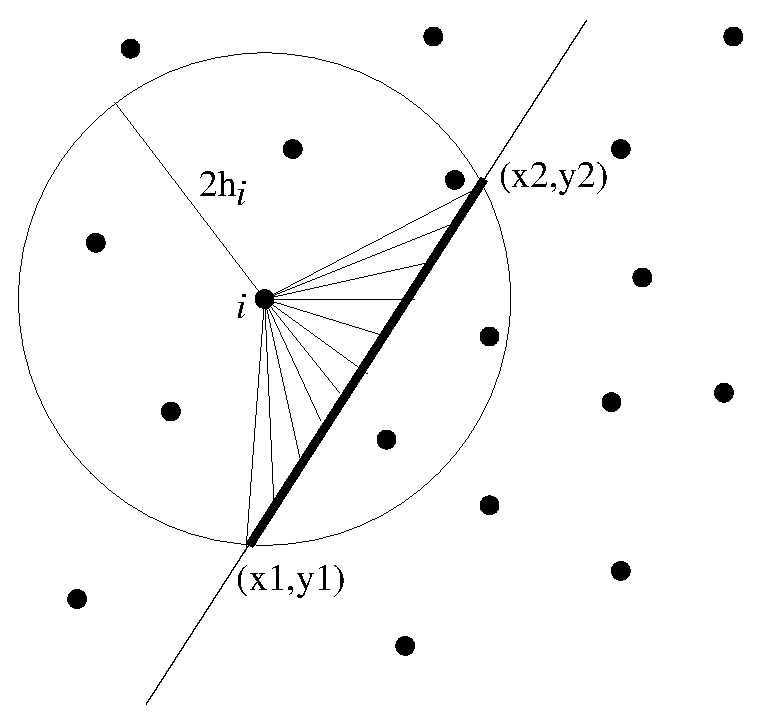
\epsfig{file=xsec2D.eps,width=0.5\textwidth}
\caption{Computation of a one dimensional cross section through 2D data}
\label{fig:xsec2D}
\end{center}
\end{figure}
 
 An example of a 1D cross section through 2D data is shown in Figure
\ref{fig:xsec2Dexample}.
\begin{figure}
\begin{center}
%%\begin{turn}{270}\epsfig{file=xsec2Dexample.ps,height=\textwidth}\end{turn}
%%\label{fig:xsec2Dexample}
\end{center}
\end{figure}

 In principle a similar method could be used for oblique cross sections
through 3D data. In this case we would need to find the intersection
between the smoothing sphere and the cross section plane. However
in 3D it is simpler just to rotate the particles first and then take
a straight cross section as described above.

\subsection{Rendering of 3D data}
 In three dimensions we must take either a projection through the whole domain or a cross section slice.
 
\subsubsection{Projections} 
 In the projection case the interpolation is similar to the 2D case, that is the interpolant is
given by
\begin{equation}
\phi(x,y) = \sum_b m_b \frac{\phi_b}{\rho_b} Y(x - x_b, y-y_b, h_b).
\end{equation}
In this case, however, the kernel (denoted $Y$) is the usual cubic spline but integrated through one spatial
dimension. This results in a map of the rendered quantity integrated along the line of sight.
In the case of vector quantities each component is interpolated separately, giving a vector
map which is also integrated along the line of
sight.

\subsubsection{Cross sections of 3D data}
 A cross section can be taken of SPH data by summing the
contributions to each pixel in the cross section plane from all particles within
$2h$ of the plane. In
the implementation used in SUPERSPHPLOT the cross section is always at a fixed value of the third co-ordinate
(ie. for xy plots the cross section is in the z direction). Oblique cross
sections can be taken by rotating the particles first. Vector cross sections are taken by
interpolating each component separately.

 Note that the cross section position can be moved up (towards the observer) or down (away from the
 observer) through the data interactively using
the 'd' (for down) and 'u' (for up) keys in interactive mode.

\begin{figure}
\begin{center}
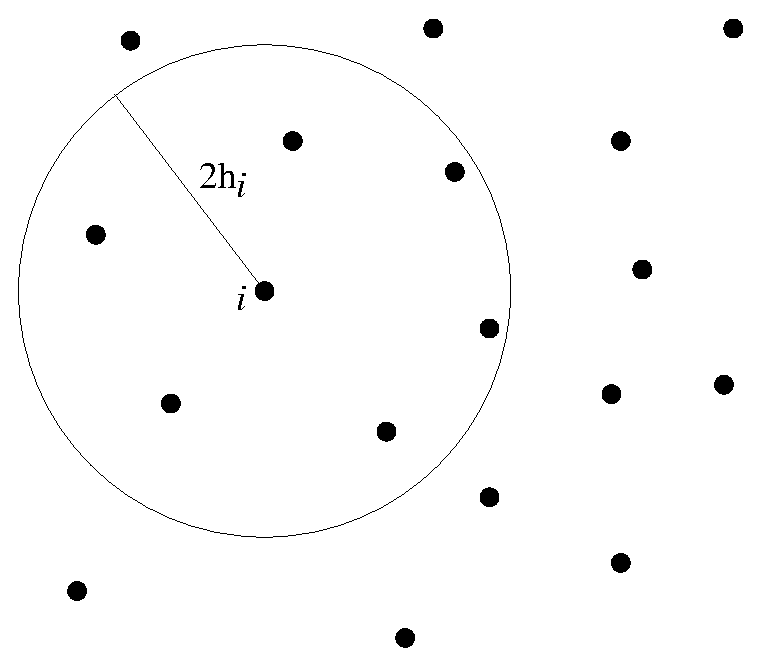
\epsfig{file=xsec3D.eps,width=0.5\textwidth}
\caption{Computation of a two dimensional cross section through 3D data}
\label{fig:xsec3D}
\end{center}
\end{figure}

\paragraph{Flythru}
 With the cross section option chosen in 3D, a flythru may be chosen at the plotting prompt. This
plots multiple slices through the data.

\section{Other features}

\subsection{Rotation}
 Rotation is achieved by tranforming to cylindrical co-ordinates about each axis, incrementing the
azimuthal angle appropriately and transforming back to cartesians. Rotated axes or boxes can be
plotted using the rotation options in the x)sec/rotate submenu, giving 3D perspective. Rotation can also be set
interactively (press 'h' in interactive mode to see the exact keystrokes). 

\subsection{Plot titles}
\label{sec:title}
 Plots may be titled individually by creating a file called \verb+titlelist+ in
the current directory, with the title on each line corresponding to the position
of the plot on the page. Thus the title is the same between timesteps unless the
steps are plotted together on the same physical page. Leave blank lines for
plots without titles. For example, creating a file called \verb+titlelist+ in
the current directory, containing the text:
\begin{verbatim}
plot one
plot two
plot three
\end{verbatim}
and positioning the title using the default options, produces the titles shown
on the graph in Figure~\ref{fig:titleexample} (where there are 6 plots on the physical page).

%%\begin{figure}
%\centering
%
%\caption{Example use of plot titles}
%\label{fig:titleexample}
%\end{figure}

\subsection{Plot legends}
\label{sec:legend}
 The text (e.g. `\verb+t=+') used in the legend can be changed via
the legend options in the (p)age submenu. The numerical value is taken from the \verb+time+ array
in the data read.

\subsection{Power spectrums (1D only)}
 In one dimension an extra plot item appears
in the data menu which takes a power spectrum (in space) of a particular
variable defined on the particles. Upon selection the user is prompted for
various settings before plotting the power spectrum. For data defined on
irregularly distributed particles, there are two methods for taking the power
spectrum: Either to interpolate to an even grid and use a Fourier
transform or to use a method for calculating a periodogram of
irregularly sampled data which can have significant advantages over
interpolation. Algorithms for both of these methods have been
implemented. For the first, the SPH data is interpolated to a one dimensional
grid using the kernel via the \verb+interpolate1D+ subroutine before calculating the (slow!) fourier
transform in \verb+powerspectrum_fourier+. For the second, an algorithm due to
Lomb and \citet{scargle81} described in \citet{numericalrecipes} is
used\footnote{Note that the subroutines given in \citet{numericalrecipes} have
\emph{not} been used as they are not free software.},
located in the subroutine \verb+powerspectrum_lomb+. The actual plotting is done
in the subroutine \verb+plot_powerspectrum+. An example of this feature is shown
in Figure~\ref{fig:powerspectrum_lomb}, where a power spectrum of a given
spectral index has been defined on the particles as an initial condition. The
plot shows the velocity variable given the initial power spectrum and the power
spectrum calculated via the Lomb periodogram.
\begin{figure}
\centering

\caption{Example of one dimensional power spectrum using the Lomb periodogram}
\label{fig:powerspectrum_lomb}
\end{figure}

 It should be stressed, however, that \emph{neither} of the subroutines for
calculating the power spectrum is particularly fast and have \emph{only} been included as a preliminary feature
since I have used them once or twice in one dimensional simulations where speed
is not an issue. The algorithms are fairly simple to extend to multidimensional
data, although faster implementations would be needed (such as a Fast
Fourier Transform routine).


\section{FAQS: How do I...}

\subsection{Read/process my data into images without having to answer prompts?}
 Firstly edit the settings in the \verb+defaults+ file in the current
directory (created by doing a `save defaults' from the main menu) before invoking SUPERSPHPLOT.

 Having edited the defaults file, the simplest way of running SUPERSPHPLOT
non-interactively is to write a small shell script which runs SUPERSPHPLOT
and answers the prompts appropriately. Something like the following should work:
\begin{verbatim}
#!/usr/bin/tcsh
cd plot
supersphplot myrun* << ENDINPUT
2
1
8
0
mypostcript.ps/ps
q
ENDINPUT
\end{verbatim}
which would plot the data in columns 2 and 1 and render the data in column 8 with
output to file \verb+mypostscript.ps+.

\subsection{Calculate additional quantities?}
 Additional quantities are calculated in the subroutine \verb+calc_quantities+,
in which it should be a simple matter to add your own.
If the calculated quantity is to be used elsewhere (for example in an exact
solution), an indicator should be created for its position in the data array
(e.g. the integer variable \verb+ih+ refers to the position of the smoothing
length in the data array). It is also preferable to indicate those quantities
from which the new quantity is calculated, so that no error will occur if they
are not present.

\subsection{What about boundaries? How does the rendering work near a boundary?}
 Usual practise in SPH simulations near boundaries is
to introduce ghost particles which mirror the real particles. SUPERSPHPLOT does not
explicitly setup any ghost particles but will use any that are present in the data
(specified using \verb+labeltype = 'ghost'+ in the \verb+read_data+ subroutine and
then specifying the number of particles of this type). Ghost particles contribute
to the rendering calculations but not to the determination of the plot limits. Note,
however, that SUPERSPHPLOT does \emph{not} set up ghost particles itself, as this may depend
on the type and location of the boundary. Thus if your simulation uses ghost particle
boundaries, the ghost particles should be dumped alongside the gas particles in the
output file so that their positions, masses, densities and smoothing lengths can be
read into SUPERSPHPLOT and used to render the image appropriately.

\subsection{Use special characters in the plot labels?}
 Several of the examples shown in this manual use special characters (such as
the $\int$ character) in the plot labels. The PGPLOT user guide explains how to do
this, but the basic idea is that PGPLOT uses escape sequences to plot special
characters. For example to plot the greek letter $\rho$ we would use
\begin{verbatim}
label = 'this would print the greek letter \gr'
\end{verbatim}
where \verb+\gr+ is the PGPLOT escape sequence for $\rho$. For other
characters the escape sequence is given by a number. For example for the integral 
\begin{equation}
\int v_x \mathrm{dx}
\end{equation}
we would use
\begin{verbatim}
label = '\(2268) v\d x \u dx'
\end{verbatim}
where \verb+\(2268)+ is the escape sequence for the integral sign. The
\verb+\d+ indicates that what follows should be printed as subscript and
\verb+\u+ correspondingly indicates a return to normal script (or from normal script to
superscript). All of the escape sequences for special characters are listed in
the appendix to the PGPLOT user guide.
\begin{quote}
 WARNING: Note that the use of escape characters can be compiler dependent and
 may not therefore work on all compilers.
\end{quote}

\subsection{Make movies?}
 At the PGPLOT device prompt
\begin{verbatim}
Graphics device/type (? to see list, default /xwin):
\end{verbatim}
choose \verb+/gif+ or \verb+/vgif+ (some installations of PGPLOT may also have \verb+/png+
installed). The images will then be written as \verb+.gif+ files which can then be easily compiled
together to form an animation. Under unix the \verb+gifmerge+ command (if installed) is a simple way
of making a single animated gif file out of a series of gif images. Animated gifs are robust but
require large amounts of memory to run at any reasonable speed. However many software packages exist
for converting animated gifs into other, more compressed formats (such as the windows .avi format or
under unix the .fli format\footnote{Note that MPEG is a particularly poor choice for simulation data}). One such package is the
\verb+convert+ command included as part of the GIMP (Gnu Image Manipulation Package) toolkit.
For presentations the windows .avi format is a good choice, although codecs for conversion are a
little harder to come by. Under windows the commercially available \verb+videomach+ program is one
such tool as well as several Microsoft products.

 Another tool under unix is the \verb+fbm2fli+ package, which will take a series of .gif or .png files and
convert them into a .fli animation (which can be played, for example by the \verb+xanim+ tool). This
format is great for animations of simulations but as yet does not import into powerpoint and the like.

\section{User contributions / Wishlist for future improvements}
 Please contribute!! Any user contributions and/or suggestions would be greatly
appreciated. The following in particular would be very useful:

\begin{itemize}
\item Exact solutions for your favourite test problem(s). It would be great to
build a library of user-contributed exact solutions.
\item Data analysis tools (e.g. fourier transforms / statistical analysis /
algorithms for finding binary stars etc) which could be incorporated.
\item New visualisation techniques (e.g. an isosurfacing routine for SPH, better
vortex line tracing).
\item More colour schemes (see \verb+colours.f90+ for how to do this)
\item Pretty pictures! If you happen to plot some of your data and spend the
next several minutes marvelling at how astoundingly beautiful it all looks, please send
me a copy (either ps, gif or a movie) to add to the gallery and a few lines
describing the simulation.
\end{itemize}


If you wish to send me subroutines or snippets of (Fortran only!) code for doing any of the above or
more, please also send me a \LaTeX file
documenting the subroutine similar to the documentation given in this user guide.
Also, please, please comment your code clearly so that others can figure out
what it does and try to catch as many errors as possible so that the whole
program is robust.  One thing I have avoided doing is to use any SPH
routines which explicitly require finding neighbours, to avoid introducing treecodes and
the like and to keep the program independent of any particular implementation of
SPH. An example of a
routine would be to find the div/curl of a vector quantity using
the SPH summation.

Contributions, comments and inevitable bug fixes
should be sent to:
\begin{verbatim}
dprice@astro.ex.ac.uk
\end{verbatim}
although check that this email address is current because I am still a postdoc!

\section*{Acknowledgements}
 Several of the routines were developed from ideas used by Matthew Bate. The
polytrope exact solution is from a routine by Joe Monaghan. I am indebted to one
Thomas S. Ullrich at the University of Heidelberg who wrote the prompting module
which is used throughout the program.

\newpage
\appendix

\section{Source code overview}
Here is a brief description of all the files making up the code:
\begin{longtable}{|lp{0.7\textwidth}|}
\hline
Filename & Description \\
\hline \endhead
\multicolumn{2}{|r|}{\emph{continued on next page}} \\
\hline \endfoot
\hline \endlastfoot
     allocate.f90           & allocates memory for main arrays \\
     calc\_quantities.f90    & calculates additional quantities from particle data \\
     colours.f90            & colour schemes for rendering\\
     colourparts.f90	 & colours particles\\
     danpgsch.f           & sets character height independent of page size\\
     danpgtile.f          & my utility for tiling plots on the pgplot page\\
     danpgwedg.f          & my very minor modification of pgwedg\\
     defaults.f90           & writes/reads default options to/from file\\
     exact.f90              & module handling exact solution settings\\
     exact\_fromfile.f90     & reads an exact solution tabulated in a file\\
     exact\_mhdshock.f90     & some tabulated solutions for mhd shocks\\ 
     exact\_polytrope.f90    & exact solution for a polytrope\\
     exact\_rhoh.f90	 & exact relation between density and smoothing length\\
     exact\_sedov.f90        & exact solution for sedov blast wave\\
     exact\_shock.f90        & exact solution for hydrodynamic shocks\\
     exact\_wave.f90         & exact solution for a propagating sine wave\\
     exact\_toystar.f90      & exact solution for the toy star problem\\
     exact\_toystar2D.f90    & exact solution for the 2D toy star problem\\
     get\_data.f90           & wrapper for main data read\\
     geometry.f90           & module handling different coordinate systems\\
     globaldata.f90         & various modules containing "global" variables\\
     interactive.f90        & drives interactive mode\\
     interpolate1D.f90	 & interpolation of 1D SPH data to grid using kernel\\
     interpolate2D.f90	 & interpolation of 2D SPH data to grid     \\
     interpolate3D\_xsec.f90 & 3D cross section interpolations\\
     interpolate3D\_projection.f90	 & 3D interpolation integrated through domain\\
     legends.f90		       & plots (time) legend on plot\\
     limits.f90                   & sets initial plot limits and writes to/reads from limits file\\
     menu.f90               & main menu\\
     options\_data.f90       & sets options relating to current data\\
     options\_limits.f90     & sets options relating to plot limits\\
     options\_page.f90       & sets options relating to page setup\\
     options\_particleplots.f90 & sets options relating to particle plots\\
     options\_powerspec.f90  & sets options for power spectrum plotting\\
     options\_render.f90	 & sets options for render plots\\
     options\_vector.f90	 & sets options for vector plots\\
     options\_xsecrotate.f90 & sets options for cross sections and rotation\\
     particleplot.f90       & subroutines for particle plotting\\
     plot\_powerspectrum.f90 & calls powerspectrum and plots it\\
     plotstep.f90           & main subroutines which drive plotting of a single timestep\\
     powerspectrums.f90     & calculates power spectrum of 1D data (2 methods)\\
     read\_data\_dansph.f90   & reads data from my format of data files\\
     read\_data\_mbate.f90    & reads data from matthew bate's format of data files\\
     read\_data\_xxx.f90 & reads data from \ldots \\ 
     render.f90	 	 & takes array of pixels and plots render map/contours etc\\
     rotate.f90             & subroutines controlling rotation of particles\\
     setpage.f90            & sets up the PGPLOT page (replaces call to PGENV/PGLAB)\\
     supersphplot.f90	 & main program, drives menu loop\\
     timestepping.f90       & controls stepping through timesteps\\
     titles\_read.f90        & reads a list of titles to be used to label each timestep\\
     transform.f90	 	 & applies various transformations to data (log10, 1/x, etc) \\
\end{longtable}

\section{Exact solutions}
\label{sec:exact}
\subsection{Shock tubes (Riemann problem)}
 The subroutine \verb+exact_shock+ plots the exact solution for a one-dimensional shock tube
(Riemann problem). The difficult bit of the problem is to determine the jump in
pressure and velocity across the shock front given the initial left and right
states. This is performed in a separate subroutine (riemannsolver) as there are 
many different methods by which this can be done (see e.g. \citealt{toro92}). 
The actual subroutine exact\_shock reconstructs the shock profile (consisting of
a rarefaction fan, contact discontinuity and shock, summarised in Figure
\ref{fig:shocktube}), given the post-shock values of pressure and
velocity. 

 The speed at which the shock travels into the `right' fluid can be computed from the post shock
velocity using the relation
\begin{equation}
v_{shock} = v_{post}\frac{(\rho_{post}/\rho_R)}{(\rho_{post}/\rho_R)- 1},
\end{equation}
where the jump conditions imply
\begin{equation}
\frac{\rho_{post}}{\rho_R} = \frac{(P_{post}/P_R) + \beta}{1 + \beta (P_{post}/P_R)}
\end{equation}
with
\begin{equation}
\beta = \frac{\gamma - 1}{\gamma + 1}.
\end{equation}

\subsubsection{Riemann solver}
 The algorithm for determining the post-shock velocity and pressure is taken
from \citet{toro92}.

\subsection{Polytrope}
 The subroutine \verb+exact_polytrope+ computes the exact solution for a static polytrope with
arbitrary $\gamma$. From Poisson's equation
\begin{equation}
\nabla^2 \phi = 4\pi G \rho,
\end{equation}
assuming only radial dependence this is given by
\begin{equation}
\frac{1}{r^{2}} \frac{d}{dr} \left(r^{2} \frac{d\phi}{dr} \right) = 4\pi G \rho(r).
\label{eq:poissonsph}
\end{equation}
  
  The momentum equation assuming an equilibrium state (${\bf v} = 0$) and a
polytropic equation of state $P = K\rho^{\gamma}$ gives
\begin{equation}
\frac{d\phi}{dr} = - \frac{\gamma K}{\gamma-1}\frac{d}{dr} \left[\rho^{(\gamma -1)} \right]
\label{eq:polyk}
\end{equation}
Combining (\ref{eq:poissonsph}) and (\ref{eq:polyk}) we obtain an equation for the density profile
\begin{equation}
\frac{\gamma K}{4\pi G (\gamma - 1)} \frac{1}{r^{2}} \frac{d}{dr} \left[r^{2}
\frac{d}{dr}\left( \rho^{\gamma-1} \right) \right] + \rho(r) = 0.
\label{eq:dens}
\end{equation}
This equation can be rearranged to give
\begin{equation}
\frac{\gamma K}{4\pi G (\gamma - 1)} \frac{d^2}{dr^2}
\left[r\rho^{\gamma-1}\right] + r\rho = 0.
\end{equation}
 The program solves this equation numerically by defining a variable
\begin{equation}
\mathcal{E} = r \rho^{\gamma-1}
\end{equation}
and finite differencing the equation according to
\begin{equation}
\frac{\mathcal{E}^{i+1} - \mathcal{E}^i + \mathcal{E}^{i-1}}{(\Delta r)^2} =
\frac{4\pi G (\gamma - 1)}{\gamma K} r
\left(\frac{\mathcal{E}}{r}\right)^{1/(\gamma-1)}.
\end{equation}

\subsection{Linear wave}
 The subroutine \verb+exact_wave+ simply plots a sine function on a given graph.
 The function is of the form
\begin{equation}
y = \sin{(k x - \omega t)}
\end{equation}
where $k$ is the wavenumber and $\omega$ is the angular frequency. These
parameters are set via the input values of wavelength $\lambda = 2\pi/k$ and
wave period $P = 2\pi/\omega$.

\begin{table}
\centering
\begin{tabular}{|l|l|}
\hline
$\lambda$ & wavelength \\
$P$ & period \\
\hline
\end{tabular}
\caption{Input parameters for the linear wave exact solution}
\end{table}

\subsection{Sedov blast wave}
 The subroutine \verb+exact_sedov+ computes the self-similar Sedov solution for a blast wave.

\subsection{Toy stars}
 The subroutine \verb+exact_toystar1D+ computes the exact solutions for the `Toy
Stars' described in \citet{mp04}. The system is one dimensional with velocity $v$, density $\rho$, and pressure
$P$. The acceleration equation is 
\begin{equation}
\frac{dv}{dt} = - \frac{1}{\rho} \frac{\partial P}{\partial x}  - \Omega^2 x,
\end{equation}
 We assume the equation of state is 
\begin{equation}
P = K \rho^\gamma,
\end{equation} 

 The exact solutions provided assume the equations are scaled such that
$\Omega^2 = 1$.
 
\subsubsection{Static structure}
The static structure is given by
\begin{equation}
\bar \rho = 1- x^2,
\end{equation}

\subsubsection{Linear solutions}
The linear solution for the velocity is given by
\begin{equation}
v = 0.05 C_s G_n(x) \cos{\omega t} )
\end{equation}
density is
\begin{equation}
\rho = \bar{\rho} + \eta
\end{equation}
where 
\begin{equation}
\eta = 0.1 C_s \omega P_{n+1}(x) \sin{(\omega t)})
\end{equation}

\subsubsection{Non-linear solution}
In this case the velocity is given by
\begin{equation}
v = A(t) x,
\end{equation}
whilst the density solution is
\begin{equation}
\rho^{\gamma -1} = H(t) - C(t) x^2.
\end{equation}
where the parameters A, H and C are determined by solving the ordinary
differential equations
\begin{eqnarray}
\dot{H} & = & -AH(\gamma -1), \\
\dot{A} & = & \frac{2K \gamma}{\gamma -1} C - 1 - A^2 \\
\dot{C} & = & -AC(1+ \gamma),
\end{eqnarray}
The relation
\begin{equation}
A^2 = -1 - \frac{2 \sigma C}{\gamma -1} + kC^{\frac{2}{\gamma +1}},
\label{eq:kconst}
\end{equation}
is used to check the quality of the solution of the differential equations by
evaluating the constant $k$ (which should remain close to its initial value).

\subsection{MHD shock tubes}
 These are some tabulated solutions for specific MHD shock tube problems at a
given time taken from the tables given in \citet{dw94} and \citet{rj95}.

\subsection{h vs $\rho$}
 The subroutine exact\_hrho simply plots the relation between smoothing length
and density, ie.
\begin{equation}
h = h_{fact} \left(\frac{m}{\rho}\right)^{1/\nu}
\end{equation}
where $\nu$ is the number of spatial dimensions. The parameter $h_{fact}$ is
output by the code into the header of each timestep. For particles of different
masses, a different curve is plotted for each different mass value.

\newpage

\section{Writing your own read\_data subroutine}
\label{sec:writeyourown}
The first \verb+ndim+ columns in the main data array \emph{must} contain the particle co-ordinates.
After these columns the ordering of data is not important, although vector quantities should
always be listed with components in the correct order (e.g. $(\nabla\times {\bf v})_x$,
followed by the $y-$ and $z-$ components) for both vector plotting and for the
correct co-ordinate transformation of the vector quantities. Note that the co-ordinates and velocities can have different
numbers of dimensions (specified by \verb+ndim+ and \verb+ndimV+) since this can occur, for example, in MHD simulations.

Most important is that, for the rendering routines to work, the density, particle
masses and smoothing lengths for \emph{all} of the (gas) particles \emph{must} be read in from
the data file and their locations in the main data array labelled using the integer
parameters \verb+irho+, \verb+ipmass+ and \verb+ih+. Labelling of the location of other particle
quantities (e.g. \verb+iutherm+ for the thermal energy) is used in
order to plot the exact solutions on the appropriate graphs and also for calculating
additional quantities (e.g. calculation of the pressure uses \verb+iutherm+ and
\verb+irho+).

 The positions of vector components in the data columns are indicated by setting the variable \verb+iamvec+ of that
column equal to the first component of the vector of which this component is a part. So if column 4
is a vector quantity (say ${\bf v}$ in 3D), then \verb+iamvec(4) = 4+, \verb+iamvec(5) = 4+ and
\verb+iamvec(6) = 4+. Similarly the string \verb+labelvec+ should be set, ie. \verb+labelvec = 'v'+ for these columns.

\bibliographystyle{bibstyle}
\bibliography{sph,mhd}

\end{document}
